\chapter{Cristallographie et diffraction des rayons X}\label{ch:b3:x-ray-diffraction}

En 1912, un faisceau de rayons X envoyé à travers un cristal de sulfate de
cuivre laissa sur une plaque photographique une figure de taches nettes~:
les cristaux diffractent les rayons X comme un réseau diffracte la
lumière, parce que les distances entre leurs atomes sont comparables à la
longueur d'onde des rayons X. Un an plus tard, William Lawrence Bragg,
alors étudiant, lut sur de telles figures la structure du sel gemme ---
et montra que le solide ne contient aucune molécule \ce{NaCl}, mais
seulement un réseau dans lequel chaque ion a six voisins de l'autre
espèce. Toutes les structures cristallines citées dans le volume de
première année et dans ce livre ont été trouvées de cette façon. Ce
chapitre donne la géométrie des réseaux et de leur symétrie, la condition
de diffraction, les intensités qui révèlent le contenu de la maille, et
les méthodes sur poudre et sur monocristal employées dans tous les
laboratoires.

\begin{recall}
Le volume de première année a décrit les cristaux par un réseau de
nœuds, un motif et une maille avec ses paramètres de maille~; il a
compté la multiplicité d'une maille, construit les structures cubique à
faces centrées, cubique centrée et hexagonale compacte et les types sel
gemme, chlorure de césium, blende et fluorine~; il a calculé une masse
volumique à partir d'une maille. Le \Cref{ch:b3:point-groups} a défini
les \omterm{def:b3:point-groups:operation}{opérations de symétrie} et les \omterm{def:b3:point-groups:point-group}{groupes ponctuels}.
\end{recall}

\begin{omfigure}
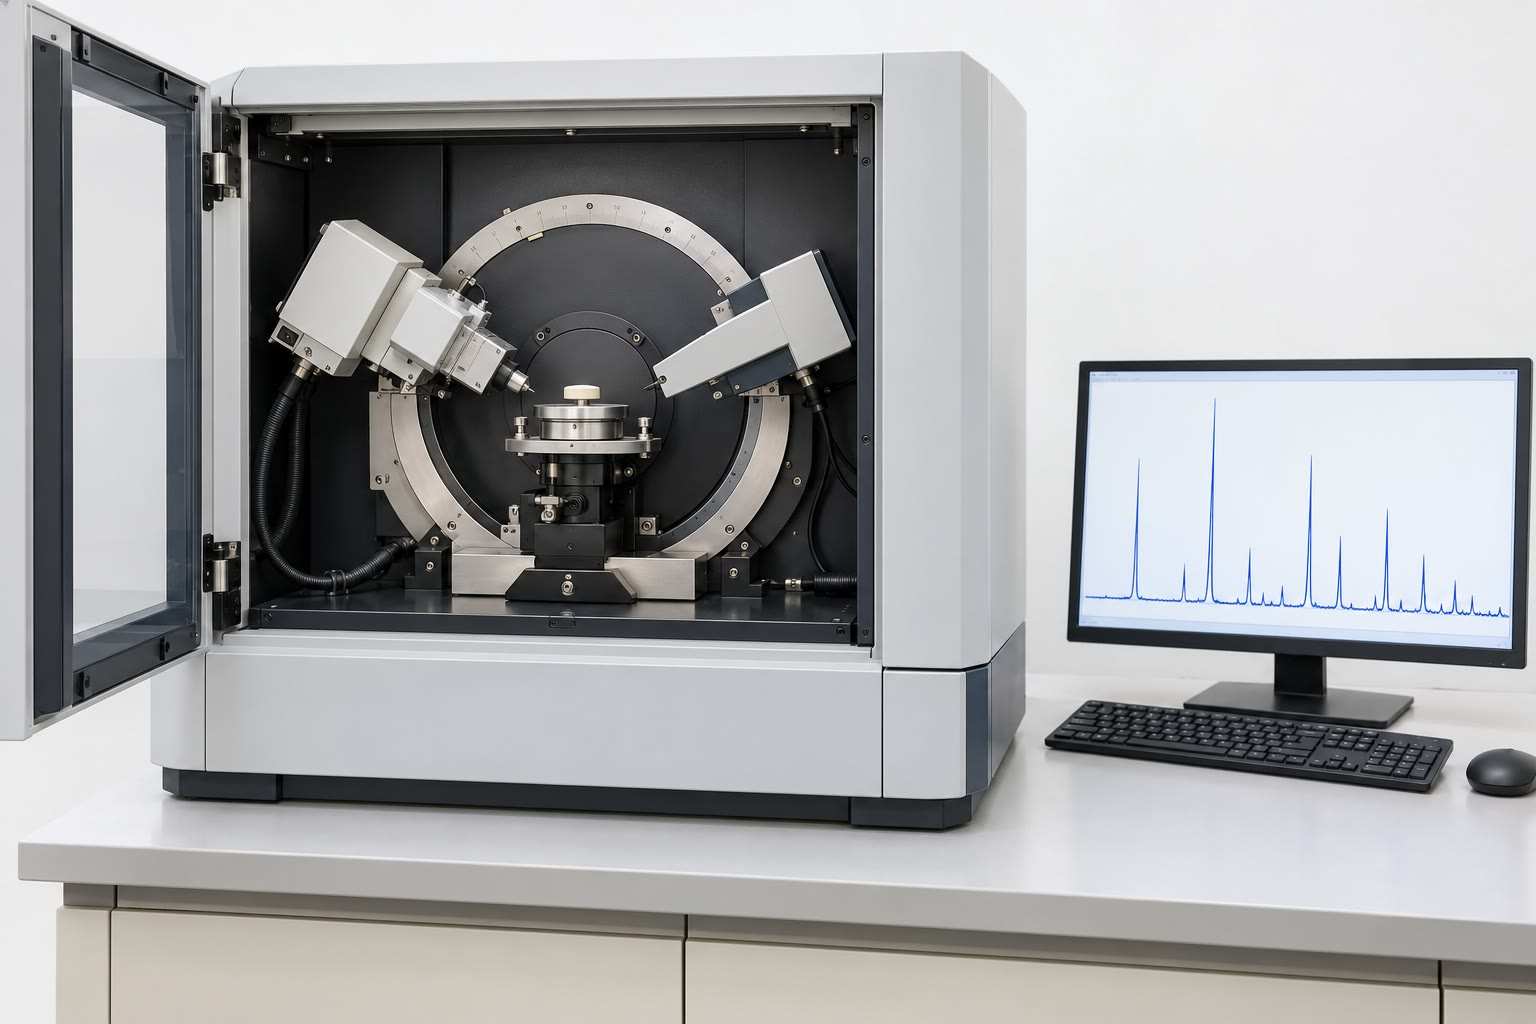
\includegraphics[width=0.6\linewidth]{images/book4/ai/b3-09-diffractometer.jpg}

{\small Un diffractomètre de poudre de paillasse~: le tube à rayons X et
le détecteur tournent sur un cercle autour de l'échantillon plan.}
\end{omfigure}

\section{Systèmes cristallins et réseaux de Bravais}

Un réseau ne peut avoir que des \omterm{def:b3:point-groups:operation}{opérations de symétrie} qui l'envoient sur
lui-même. Cela les restreint sévèrement.

\begin{theorem}[La restriction cristallographique]\label{thm:b3:x-ray-diffraction:restriction}
Les seuls axes de rotation compatibles avec un réseau sont d'ordre 1, 2,
3, 4 et 6.
\end{theorem}

\begin{proof}
Dans une base de vecteurs du réseau, une rotation de symétrie envoie les
vecteurs du réseau sur des vecteurs du réseau, donc sa matrice a des
coefficients entiers et une trace entière. La trace ne dépend pas de la
base~; dans une base orthonormée où $z$ est porté par l'axe, elle vaut
$1 + 2\cos\theta$. Donc $2\cos\theta$ est un entier compris entre $-2$
et 2~:
$\cos\theta \in \{-1, -\frac12, 0, \frac12, 1\}$, $\theta = 180^\circ, 120^\circ, 90^\circ,
60^\circ, 0^\circ$~: ordres 2, 3, 4, 6, 1. Un axe d'ordre cinq est
impossible.
\end{proof}

\begin{definition}[Système cristallin, réseau de Bravais, mode de réseau]\label{def:b3:x-ray-diffraction:crystal-system}
Les réseaux se répartissent selon leur symétrie en sept \emph{systèmes
cristallins}\index{systeme cristallin@système cristallin} (triclinique,
monoclinique, orthorhombique, quadratique, trigonal, hexagonal,
cubique). Une maille peut porter des nœuds seulement à ses sommets
(primitive, P), ou aussi en son centre (centrée, I), aux centres de
toutes ses faces (à faces centrées, F) ou d'une seule paire de faces
(à bases centrées, C), ou sur une grande diagonale (rhomboédrique, R)~:
c'est son \emph{mode de réseau}\index{mode de reseau@mode de réseau}.
Les 14 combinaisons distinctes d'un système et d'un mode sont les
\emph{réseaux de Bravais}\index{reseau de Bravais@réseau de Bravais}.
\end{definition}

\begin{center}\small
\begin{tabular}{lll}
\hline
système & contraintes sur la maille & modes \\ \hline
triclinique & aucune & P \\
monoclinique & $\alpha = \gamma = 90^\circ$ & P, C \\
orthorhombique & $\alpha = \beta = \gamma = 90^\circ$ & P, C, I, F \\
quadratique & $a = b$, tous les angles à $90^\circ$ & P, I \\
trigonal & $a = b = c$, $\alpha = \beta = \gamma \ne 90^\circ$ (axes rhomboédriques) & R \\
hexagonal & $a = b$, $\alpha = \beta = 90^\circ$, $\gamma = 120^\circ$ & P \\
cubique & $a = b = c$, tous les angles à $90^\circ$ & P, I, F \\ \hline
\end{tabular}
\end{center}

\begin{omfigure}
\tdplotsetmaincoords{60}{100}
\begin{tikzpicture}[tdplot_main_coords, scale=1.25, font=\small]
  \foreach \s/\lab in {0/{cubique P}, 3.0/{cubique I}, 6.0/{cubique F}}{
    \begin{scope}[xshift=\s cm]
      \pic[transform shape] {omcubeo={1.6}};
      \foreach \x in {0,1.6}{\foreach \y in {0,1.6}{\foreach \z in {0,1.6}{\node[cellA=2.6mm] at (\x,\y,\z) {};}}}
      \node[anchor=north] at (0.8,0.8,-0.62) {\lab};
    \end{scope}}
  \begin{scope}[xshift=3.0cm]
    \node[cellB=2.6mm] at (0.8,0.8,0.8) {};
  \end{scope}
  \begin{scope}[xshift=6.0cm]
    \foreach \p in {(0.8,0.8,0),(0.8,0.8,1.6),(0.8,0,0.8),(0.8,1.6,0.8),(0,0.8,0.8),(1.6,0.8,0.8)}{\node[cellB=2.6mm] at \p {};}
  \end{scope}
\end{tikzpicture}

{\small Les trois \omterm{def:b3:x-ray-diffraction:crystal-system}{réseaux de Bravais} cubiques~: primitif (nœuds aux
sommets), centré (plus le centre, en rouge) et à faces centrées (plus
les six centres des faces, en rouge). Leurs mailles contiennent 1, 2 et
4 nœuds.}
\end{omfigure}

\section{Plans réticulaires et réseau réciproque}

\begin{definition}[Plan réticulaire, indices de Miller, distance interréticulaire]\label{def:b3:x-ray-diffraction:miller}
Un \emph{plan réticulaire}\index{plan reticulaire@plan réticulaire} est un
plan passant par au moins trois nœuds non alignés~; il appartient à une
famille de plans parallèles et équidistants qui contiennent tous les
nœuds. Si le plan de la famille le plus proche de l'origine coupe les
axes en $a/h$, $b/k$, $c/l$, les entiers $(hkl)$, sans facteur commun,
sont ses \emph{indices de Miller}\index{indices de Miller} (un indice 0
pour un plan parallèle à un axe). La distance entre deux plans voisins
est la \emph{distance interréticulaire}\index{distance interreticulaire@distance interréticulaire} $d_{hkl}$.
\end{definition}

\begin{proposition}[Distances dans les mailles orthogonales]\label{prop:b3:x-ray-diffraction:spacing}
Pour une maille orthorhombique, $\dfrac{1}{d_{hkl}^2} = \dfrac{h^2}{a^2} + \dfrac{k^2}{b^2} +
\dfrac{l^2}{c^2}$~; pour une maille cubique, $d_{hkl} = a/\sqrt{h^2 + k^2 + l^2}$.
\end{proposition}

\begin{proof}
Le plan $hx/a + ky/b + lz/c = 1$ a pour vecteur normal $\mathbf n = (h/a, k/b, l/c)$
et se trouve à la distance $1/|\mathbf n|$ de l'origine~; le plan
parallèle passant par l'origine appartient à la famille, donc
$d = 1/|\mathbf n|$.
\end{proof}

\begin{definition}[Réseau réciproque]\label{def:b3:x-ray-diffraction:reciprocal}
Pour un réseau de vecteurs de base $\mathbf a$, $\mathbf b$, $\mathbf c$ et
de volume de maille $V$,
le \emph{réseau réciproque}\index{reseau reciproque@réseau réciproque} a pour vecteurs de base
$\mathbf a^* = (\mathbf b\times\mathbf c)/V$, $\mathbf b^* = (\mathbf c\times\mathbf a)/V$,
$\mathbf c^* = (\mathbf a\times\mathbf b)/V$, de sorte que $\mathbf a\cdot\mathbf a^* = 1$ et
$\mathbf a\cdot\mathbf b^* = 0$. Son nœud $\mathbf G_{hkl} = h\mathbf a^* + k\mathbf b^* + l\mathbf c^*$
est perpendiculaire aux plans $(hkl)$, et $|\mathbf G_{hkl}| = 1/d_{hkl}$.
\end{definition}

\section{La diffraction}

\begin{theorem}[Loi de Bragg]\label{thm:b3:x-ray-diffraction:bragg}
Des rayons X de longueur d'onde $\lambda$ ne sont réfléchis par une
famille de plans d'équidistance $d$ que sous les angles rasants $\theta$
qui vérifient
\[
2d\sin\theta = n\lambda, \qquad n = 1, 2, \dots,
\]
c'est la \emph{loi de Bragg}\index{loi de Bragg}. On absorbe l'ordre $n$
en notant la réflexion $(nh\,nk\,nl)$, de distance $d/n$.
\end{theorem}

\begin{proof}
Les rayons diffusés par deux plans voisins, sous des angles d'incidence
et de réflexion égaux à $\theta$, présentent une différence de marche de
$2d\sin\theta$ (les deux segments situés de part et d'autre de la
normale passant par le plan inférieur). Ils se renforcent quand cette
différence est un nombre entier de longueurs d'onde~; avec des millions
de plans, tout autre angle donne des rayons qui s'annulent deux à deux.
\end{proof}

\begin{omfigure}
\begin{tikzpicture}[font=\small, >=Stealth]
  \foreach \y in {0,-1.1}{\draw[thick] (-0.4,\y) -- (7.4,\y);}
  \foreach \x in {0,1.4,...,7.0}{\fill (\x,0) circle (1.5pt) (\x,-1.1) circle (1.5pt);}
  \draw[->, omDef, thick] (0.2,1.75) -- (2.8,0);
  \draw[->, omDef, thick] (2.8,0) -- (5.4,1.75);
  \draw[->, omDef, thick] (-1.43,1.75) -- (2.8,-1.1);
  \draw[->, omDef, thick] (2.8,-1.1) -- (7.03,1.75);
  \draw[densely dashed] (2.8,0) -- (2.8,-1.1);
  \draw[omThm, thick] (2.8,0) -- (2.18,-0.68) (2.8,0) -- (3.42,-0.68);
  \draw[omThm, very thick] (2.18,-0.68) -- (2.8,-1.1) -- (3.42,-0.68);
  \draw (1.8,0) arc[start angle=180, end angle=213.9, radius=1.0];
  \node[anchor=east] at (1.85,-0.2) {$\theta$};
  \draw[<->] (7.7,0) -- (7.7,-1.1) node[midway, right] {$d$};
  \node[omThm, anchor=north] at (2.8,-1.2) {différence de marche $2d\sin\theta$};
\end{tikzpicture}

{\small La construction de Bragg. Les rayons réfléchis par des plans
voisins parcourent en plus les deux segments rouges, de $d\sin\theta$
chacun~; les ondes se renforcent quand
$2d\sin\theta$ est un nombre entier de longueurs d'onde.}
\end{omfigure}

\begin{proposition}[Condition de Laue]\label{prop:b3:x-ray-diffraction:laue}
Avec des vecteurs d'onde incident et diffusé $\mathbf k$ et $\mathbf k'$
de norme
$1/\lambda$, il y a diffraction quand $\mathbf k' - \mathbf k = \mathbf G_{hkl}$,
un vecteur du \omterm{def:b3:x-ray-diffraction:reciprocal}{réseau réciproque}~; cette condition équivaut à la \omterm{thm:b3:x-ray-diffraction:bragg}{loi de
Bragg}.
\end{proposition}

\begin{proof}
Les ondes diffusées par deux nœuds séparés par un vecteur du réseau
$\mathbf R$ sont déphasées de $2\pi(\mathbf k' - \mathbf k)\cdot\mathbf R$~;
elles se renforcent toutes si ce déphasage est un multiple de $2\pi$
pour tout $\mathbf R$, c'est-à-dire si $\mathbf k' - \mathbf k$ appartient
au \omterm{def:b3:x-ray-diffraction:reciprocal}{réseau réciproque} (d'après la
définition $\mathbf a\cdot\mathbf a^* = 1$, $\mathbf a\cdot\mathbf b^* = 0$\dots).
Pour une diffusion élastique,
$|\mathbf k| = |\mathbf k'|$ et $|\mathbf k' - \mathbf k| = 2\sin\theta/\lambda$,
où $2\theta$ est l'angle qu'ils forment~; avec $|\mathbf G| = 1/d$, on
obtient $2d\sin\theta = \lambda$, et $\mathbf G$ est normal aux plans
réflecteurs.
\end{proof}

\begin{definition}[Sphère d'Ewald]\label{def:b3:x-ray-diffraction:ewald}
La \emph{sphère d'Ewald}\index{sphere d'Ewald@sphère d'Ewald} a pour rayon
$1/\lambda$ et passe par l'origine du \omterm{def:b3:x-ray-diffraction:reciprocal}{réseau réciproque}, son centre étant
en $-\mathbf k$ par rapport à l'origine~; une réflexion se produit chaque
fois qu'un nœud du \omterm{def:b3:x-ray-diffraction:reciprocal}{réseau réciproque} se trouve sur elle.
\end{definition}

\begin{omfigure}
\begin{tikzpicture}[font=\small, >=Stealth, scale=0.9]
  \foreach \i in {-2,...,4}{\foreach \j in {-2,...,2}{\fill[black!60] (\i*1.0,\j*0.75) circle (1.3pt);}}
  \node[anchor=north east] at (0,0) {$O$};
  \draw[omDef] (-1.625,0.0) circle (1.625);
  \draw[->, omDef, thick] (-1.625,0) -- (0,0) node[midway, below] {$\mathbf k$};
  \draw[->, omThm, thick] (-1.625,0) -- (-1.0,1.5);
  \node[omThm, anchor=east] at (-1.4,0.85) {$\mathbf k'$};
  \draw[->, black, very thick] (0,0) -- (-1.0,1.5) node[pos=0.3, left] {$\mathbf G$};
  \node[anchor=north] at (-1.625,-1.75) {sphère d'Ewald, rayon $1/\lambda$};
  \draw[<->] (4.6,0) -- (4.6,0.75) node[midway, right] {$b^*$};
  \draw[<->] (3,-1.85) -- (4,-1.85) node[midway, below] {$a^*$};
\end{tikzpicture}

{\small La construction d'Ewald à deux dimensions (le cercle passe par
l'origine $O$ du \omterm{def:b3:x-ray-diffraction:reciprocal}{réseau réciproque}). Un nœud $\mathbf G$ situé sur le
cercle donne un faisceau diffracté $\mathbf k' = \mathbf k + \mathbf G$.
Ici, le cercle, de rayon choisi pour le dessin, passe par le nœud
$(-1, 2)$.}
\end{omfigure}

\section{Intensités et symétrie}

La \omterm{thm:b3:x-ray-diffraction:bragg}{loi de Bragg} donne les directions des faisceaux diffractés, qui ne
dépendent que du réseau~; leurs intensités dépendent du contenu de la
maille.

\begin{definition}[Facteur de diffusion atomique, facteur de structure]\label{def:b3:x-ray-diffraction:structure-factor}
Le \emph{facteur de diffusion atomique}\index{facteur de diffusion atomique} $f_j$ d'un
atome est l'amplitude qu'il diffuse, en unités de celle d'un électron~;
il est égal à son nombre d'électrons dans la direction incidente et
décroît aux grands angles. Le \emph{facteur de structure}\index{facteur de structure}
de la réflexion $hkl$ est
\[
F_{hkl} = \sum_jf_j\,\eu^{2\pi\iu(hx_j + ky_j + lz_j)},
\]
sommé sur les atomes de la maille, de coordonnées réduites $(x_j, y_j, z_j)$.
\end{definition}

\begin{proposition}[Intensité]\label{prop:b3:x-ray-diffraction:intensity}
L'intensité d'une réflexion est proportionnelle à $|F_{hkl}|^2$.
\end{proposition}

\begin{proof}[Démonstration partielle]
L'atome $j$ se trouve en $\mathbf r_j = x_j\mathbf a + y_j\mathbf b + z_j\mathbf c$~;
pour une réflexion,
$(\mathbf k' - \mathbf k)\cdot\mathbf r_j = hx_j + ky_j + lz_j$, donc son
onde a la phase
$2\pi(hx_j + ky_j + lz_j)$ par rapport à un atome situé à l'origine, et
l'amplitude $f_j$~:
la maille diffuse la somme $F_{hkl}$, et chaque maille la même. Une
intensité est le carré du module d'une amplitude. On admet que la
diffusion multiple est négligeable (approximation cinématique).
\end{proof}

\begin{definition}[Extinction systématique]\label{def:b3:x-ray-diffraction:absence}
Une \emph{extinction systématique}\index{extinction systematique@extinction systématique} est une réflexion
dont le \omterm{def:b3:x-ray-diffraction:structure-factor}{facteur de structure} s'annule pour tout cristal d'un \omterm{def:b3:x-ray-diffraction:crystal-system}{mode de
réseau} ou d'une symétrie donnés, quels que soient ses atomes.
\end{definition}

\begin{proposition}[Extinctions des réseaux centrés]\label{prop:b3:x-ray-diffraction:absences}
Dans un réseau centré, les réflexions telles que $h + k + l$ est impair
sont éteintes~; dans un réseau à faces centrées, les réflexions dont les
indices $h$, $k$, $l$ sont de parités mélangées sont éteintes.
\end{proposition}

\begin{proof}
Mode I~: tout atome en $(x,y,z)$ a une copie en $(x + \frac12, y + \frac12, z + \frac12)$,
dont le facteur de phase diffère de $\eu^{\iu\pi(h+k+l)} = (-1)^{h+k+l}$~: $F = (1 +
(-1)^{h+k+l})F'$. Mode F~: les copies aux centres de trois faces donnent
le facteur $1 +
(-1)^{h+k} + (-1)^{h+l} + (-1)^{k+l}$, égal à 4 si $h$, $k$, $l$ sont
tous pairs ou tous impairs, et à 0 sinon.
\end{proof}

\begin{example}[Sel gemme et sylvite]\label{ex:b3:x-ray-diffraction:nacl-kcl}
% ledger: lat:NaCl, lat:KCl
Dans la structure du sel gemme, cations en $(0,0,0)$ et anions en
$(\frac12,0,0)$, chacun avec les translations F~: $F_{hkl} = 4[f_+ + f_-(-1)^{h+k+l}]$
pour des indices non mélangés.
Pour \ce{NaCl}, $f(\ce{Na+}) \approx 10$ et $f(\ce{Cl-}) \approx 18$~:
les réflexions à indices tous impairs
(111), (311) sont faibles mais présentes. Pour \ce{KCl}, \ce{K+} et
\ce{Cl-} ont tous deux 18
électrons~: les réflexions à indices tous impairs disparaissent presque,
et le diagramme ressemble à celui d'un réseau cubique primitif de maille
deux fois plus petite (figure ci-dessous).
\end{example}

\begin{omfigure}
\begin{tikzpicture}
\begin{axis}[name=salts, width=0.95\linewidth, height=5.2cm, xmin=20, xmax=90,
  ymin=0, ymax=2.55, ytick=\empty, axis x line=bottom, axis y line=none,
  xlabel={$2\theta$ / degré (Cu K$\alpha_1$)}, tick label style={font=\small},
  label style={font=\small}]
\addplot[omDef, thin] table[x=tt, y expr=\thisrow{NaCl}+1.35] {figdata/out/bachelor-3-xrd-powder-salts.dat};
\addplot[omThm, thin] table[x=tt, y=KCl] {figdata/out/bachelor-3-xrd-powder-salts.dat};
\node[font=\small, omDef, anchor=west] at (axis cs:79,1.9) {\ce{NaCl}};
\node[font=\small, omThm, anchor=west] at (axis cs:77,0.55) {\ce{KCl}};
\node[font=\scriptsize, anchor=south] at (axis cs:27.36,1.52) {111};
\node[font=\scriptsize, anchor=west] at (axis cs:32.1,2.25) {200};
\node[font=\scriptsize, anchor=west] at (axis cs:28.8,0.9) {200};
\node[font=\scriptsize, anchor=west] at (axis cs:41.0,0.85) {220};
\end{axis}
\end{tikzpicture}

\begin{tikzpicture}
\begin{axis}[name=met, width=0.62\linewidth, height=4.4cm, xmin=35, xmax=100,
  ymin=0, ymax=2.35, ytick=\empty, axis x line=bottom, axis y line=none,
  xlabel={$2\theta$ / degré}, tick label style={font=\small}, label style={font=\small}]
\addplot[omDef, thin] table[x=tt, y expr=\thisrow{Cu}+1.2] {figdata/out/bachelor-3-xrd-powder-metals.dat};
\addplot[omThm, thin] table[x=tt, y=W] {figdata/out/bachelor-3-xrd-powder-metals.dat};
\node[font=\small, omDef, anchor=west] at (axis cs:55,1.5) {Cu (F)};
\node[font=\small, omThm, anchor=west] at (axis cs:44,0.4) {W (I)};
\end{axis}
\begin{axis}[at={(met.east)}, anchor=west, xshift=0.7cm, width=0.36\linewidth, height=4.4cm,
  xmin=29.7, xmax=33.7, ymin=0, ymax=1.1, ytick=\empty, axis x line=bottom,
  axis y line=none, xlabel={$2\theta$ / degré}, tick label style={font=\small},
  label style={font=\small}, title={\small Scherrer}]
\addplot[black, thick] table[x=tt, y=L200] {figdata/out/bachelor-3-xrd-powder-scherrer.dat};
\addplot[omDef, thick] table[x=tt, y=L50] {figdata/out/bachelor-3-xrd-powder-scherrer.dat};
\addplot[omThm, thick] table[x=tt, y=L10] {figdata/out/bachelor-3-xrd-powder-scherrer.dat};
\end{axis}
\end{tikzpicture}

{\small Diagrammes de poudre calculés (Cu K$\alpha_1$~; facteurs de
diffusion pris égaux aux nombres d'électrons, si bien que seules les
extinctions et les grandes tendances des intensités ont un sens). En
haut~: \ce{NaCl} et \ce{KCl}~; les raies à indices tous impairs de
\ce{KCl}
disparaissent. En bas à gauche~: le cuivre (F) présente (111), (200),
(220), (311)\dots~; le tungstène
(I) présente (110), (200), (211)\dots. En bas à droite~: la raie (200) de
\ce{NaCl} pour des cristallites de 200 (noir), 50 (bleu) et 10 nm
(rouge)~: plus les cristaux sont petits, plus les raies sont larges.}
\end{omfigure}

\begin{proposition}[Loi de Friedel]\label{prop:b3:x-ray-diffraction:friedel}
En l'absence de diffusion anomale, $|F_{hkl}| = |F_{\bar h\bar k\bar l}|$~:
un diagramme de diffraction paraît centrosymétrique même quand le
cristal ne l'est pas.
\end{proposition}

\begin{proof}
Avec des $f_j$ réels, $F_{\bar h\bar k\bar l} = \sum f_j\eu^{-2\pi\iu(\dots)} = F_{hkl}^*$,
de même module.
\end{proof}

Les \omterm{def:b3:point-groups:operation}{éléments de symétrie} qui associent une rotation ou une réflexion à
une fraction d'une translation du réseau n'existent que dans les
cristaux.

\begin{definition}[Axe hélicoïdal, plan de glissement, groupe d'espace]\label{def:b3:x-ray-diffraction:space-group}
Un \emph{axe hélicoïdal}\index{axe helicoidal@axe hélicoïdal} $n_p$ associe
une rotation de $2\pi/n$ à une translation de $p/n$ de la période du
réseau le long de l'axe ($2_1$~: un demi-tour et une demi-maille). Un
\emph{plan de glissement}\index{plan de glissement} associe une réflexion
à une translation d'un demi-vecteur du réseau parallèle au plan
(glissements $a$, $b$, $c$).
Le groupe de toutes les \omterm{def:b3:point-groups:operation}{opérations de symétrie} d'un cristal,
translations comprises, est son \emph{groupe d'espace}\index{groupe d'espace}~:
il y en a 230. Sa plus petite partie à partir de laquelle les opérations
engendrent tout le cristal est l'\emph{unité asymétrique}\index{unite asymetrique@unité asymétrique}.
Un ensemble de points laissés invariants par un \omterm{def:b3:point-groups:class}{sous-groupe} des
opérations est une \emph{position de Wyckoff}\index{position de Wyckoff}~:
les positions générales n'ont aucune symétrie, les positions
particulières se trouvent sur des \omterm{def:b3:point-groups:operation}{éléments de symétrie}.
\end{definition}

\begin{proposition}[Extinctions dues à un axe hélicoïdal]\label{prop:b3:x-ray-diffraction:screw-absence}
Un axe $2_1$ parallèle à $b$ éteint les réflexions $0k0$ avec $k$ impair.
\end{proposition}

\begin{proof}
L'axe envoie $(x, y, z)$ en $(-x, y + \frac12, -z)$. Pour $h = l = 0$, les
deux atomes ont pour facteurs de phase $\eu^{2\pi\iu ky}$ et
$\eu^{2\pi\iu k(y + 1/2)} = (-1)^k\eu^{2\pi\iu ky}$~: leur somme
s'annule pour $k$ impair.
\end{proof}

\begin{method}[Lire le symbole d'un groupe d'espace]\label{met:b3:x-ray-diffraction:read-space-group}
\begin{enumerate}
  \item La première lettre est le \omterm{def:b3:x-ray-diffraction:crystal-system}{mode de réseau} (P, I, F, C, R).
  \item Les symboles suivants donnent la symétrie selon les directions
        principales~; pour le système monoclinique, la direction unique
        est $b$. Une barre de fraction signifie «~avec un plan
        perpendiculaire à cet axe~».
  \item \textit{P}$2_1/c$, le \omterm{def:b3:x-ray-diffraction:space-group}{groupe d'espace} le plus courant des
        molécules organiques~: primitif, un axe $2_1$ selon $b$, et un
        \omterm{def:b3:x-ray-diffraction:space-group}{plan de glissement} $c$ qui lui est perpendiculaire~; ces
        éléments engendrent des \omterm{def:b3:point-groups:inversion}{centres d'inversion}. Extinctions~:
        $0k0$ avec $k$ impair, $h0l$ avec $l$
        impair.
\end{enumerate}
\end{method}

\begin{omfigure}
\begin{tikzpicture}[x=3.6cm, y=3.6cm, font=\small]
  \draw (0,0) rectangle (1,1);
  \node[anchor=north] at (0.5,-0.05) {$a \rightarrow$};
  \node[anchor=east] at (-0.05,0.5) {$b \uparrow$};
  % c-glide planes perpendicular to b at y = 1/4 and 3/4 (glide along c, normal to the page): dotted
  \draw[black, line width=1.1pt, dotted] (0,0.25) -- (1,0.25) (0,0.75) -- (1,0.75);
  % 2_1 axes parallel to b at x = 0, 1/2, 1 (height z = 1/4): lines with half-arrowheads
  \foreach \x in {0,0.5,1}{
    \draw[black, line width=1pt, {Straight Barb[left]}-{Straight Barb[left]}] (\x,0.03) -- (\x,0.97);}
  \node[font=\scriptsize, anchor=west] at (0.51,0.88) {$\tfrac14$};
  % centres of inversion at the corners, edge midpoints and centre
  \foreach \p in {(0,0),(0.5,0),(1,0),(0,0.5),(0.5,0.5),(1,0.5),(0,1),(0.5,1),(1,1)}{\pic at \p {ominv};}
  % general positions: (x,y,z), (-x,y+1/2,1/2-z), (-x,-y,-z), (x,1/2-y,1/2+z)
  \pic at (0.20,0.10) {omgenpos={$+$}{0}};
  \pic at (0.80,0.60) {omgenpos={$\tfrac12{-}$}{0}};
  \pic at (0.80,0.90) {omgenpos={$-$}{1}};
  \pic at (0.20,0.40) {omgenpos={$\tfrac12{+}$}{1}};
\end{tikzpicture}

{\small Le \omterm{def:b3:x-ray-diffraction:space-group}{groupe d'espace} \textit{P}$2_1/c$ vu selon $c$ (projection sur
le plan $ab$). Pointillés~: \omterm{def:b3:x-ray-diffraction:space-group}{plans de glissement} $c$ perpendiculaires à
$b$~; demi-flèches~: axes hélicoïdaux $2_1$ parallèles à $b$ (à la
cote $z = \frac14$)~; petits cercles~: \omterm{def:b3:point-groups:inversion}{centres d'inversion}. Une position
générale à la cote $+z$ en engendre trois autres~; une virgule marque une
copie image dans un miroir (produite par le glissement ou l'inversion)~;
$\frac12{-}$ signifie la cote $\frac12 - z$.}
\end{omfigure}

\section{Méthodes sur poudre et sur monocristal}

\begin{definition}[Diagramme de diffraction sur poudre]\label{def:b3:x-ray-diffraction:powder}
Un échantillon finement broyé contient des cristallites dans toutes les
orientations~: chaque famille de plans en trouve certaines en position de
réflexion, et les faisceaux diffractés forment des cônes. L'intensité
enregistrée en fonction de $2\theta$ est son \emph{diagramme de
diffraction sur poudre}\index{diagramme de diffraction sur poudre}, une
empreinte de la phase cristalline.
\end{definition}

\begin{method}[Indexer un diagramme de poudre cubique]\label{met:b3:x-ray-diffraction:index-cubic}
\begin{enumerate}
  \item Calculer $\sin^2\theta$ pour chaque raie~; pour un cristal
        cubique, $\sin^2\theta =
        (\lambda^2/4a^2)N$ avec $N = h^2 + k^2 + l^2$.
  \item Diviser par la plus petite valeur et chercher la suite
        d'entiers~: P donne
        $N = 1, 2, 3, 4, 5, 6, 8, \dots$ (jamais 7)~; I donne
        $2, 4, 6, 8, 10, \dots$~; F donne
        $3, 4, 8, 11, 12, 16, \dots$
  \item Choisir la suite qui convient à toutes les raies~; alors
        $a = \lambda\sqrt N/(2\sin\theta)$, de préférence à partir des
        raies aux grands angles, où une erreur sur $\theta$ compte le
        moins.
\end{enumerate}
\end{method}

\begin{method}[Le nombre de groupements formulaires dans la maille]\label{met:b3:x-ray-diffraction:z-from-density}
Avec la masse molaire $M$ d'un groupement formulaire et la masse
volumique mesurée $\rho$, $Z =
\rho N_Aa^3/M$ (pour une maille cubique) doit être un nombre entier~;
cela met à l'épreuve une structure proposée.
\end{method}

\begin{proposition}[Formule de Scherrer]\label{prop:b3:x-ray-diffraction:scherrer}
Des cristallites de taille moyenne $L$ élargissent une raie de
$\beta \approx K\lambda/(L\cos\theta)$ (largeur
à mi-hauteur en radians de $2\theta$, $K \approx 0.9$).
\end{proposition}
\admitted

Au-dessous d'environ \qty{100}{nm}, l'élargissement devient mesurable~;
la formule de Scherrer, établie dans des cours plus avancés à partir de
la transformée de Fourier d'un empilement fini de plans, permet alors
d'estimer la taille des nanocristaux
(\cref{ch:b3:inorganic-materials}).

\begin{definition}[Problème de la phase, facteur R]\label{def:b3:x-ray-diffraction:refinement}
Les intensités donnent $|F_{hkl}|$, mais pas les phases des $F_{hkl}$~;
sans elles, on ne peut pas calculer la \omterm{def:b3:computational-chemistry:dft}{densité électronique} en inversant
la série de Fourier. C'est le \emph{problème de la phase}\index{probleme de la phase@problème de la phase}. Une
structure d'essai est affinée par moindres carrés jusqu'à ce que les
modules calculés et observés concordent~; le résidu
$R = \sum\big||F_o| - |F_c|\big|/\sum|F_o|$ est son \emph{facteur
R}\index{facteur R} --- quelques pour cent pour une bonne structure.
\end{definition}

Pour un monocristal, un diffractomètre mesure des milliers de
réflexions~; les méthodes directes (relations statistiques entre les
phases des réflexions intenses) donnent une première carte de \omterm{def:b3:computational-chemistry:dft}{densité
électronique} pour la plupart des petites molécules, et l'affinement
place chaque atome à quelques millièmes de nanomètre près. Les résultats
sont déposés sous forme de fichiers CIF dans des bases de données
ouvertes, d'où sont tirés les paramètres de maille cités dans cette
série.

\begin{inthelab}[Une mesure sur poudre]
La poudre est broyée dans un mortier en agate, pressée à plat dans un
porte-échantillon, et balayée de 5 à \ang{90} en $2\theta$ avec le
rayonnement Cu K$\alpha$~; un filtre de nickel élimine l'essentiel de la
raie K$\beta$. Le diagramme est comparé aux diagrammes de référence d'une
base de données, et les paramètres de maille sont affinés avec un étalon
interne comme la poudre de silicium. Les appareils à rayons X sont
capotés et verrouillés~: l'obturateur ne peut pas s'ouvrir quand la
porte est ouverte.
\end{inthelab}

\begin{history}[The Braggs, 1913]
\begin{minipage}[t]{0.72\linewidth}
Max von Laue proposa en 1912 que les cristaux diffractent les rayons X,
et Walter Friedrich et Paul Knipping enregistrèrent le premier
diagramme. William Lawrence Bragg, âgé de vingt-deux ans, expliqua les
taches comme des réflexions sur des \omterm{def:b3:x-ray-diffraction:miller}{plans réticulaires} et, avec son père
William Henry Bragg, qui construisit un spectromètre à rayons X, résolut
les structures de \ce{NaCl}, de \ce{KCl} et du diamant en 1913. Le père
et le fils partagèrent le prix Nobel de physique 1915.
\end{minipage}\hfill
\begin{minipage}[t]{0.22\linewidth}\vspace{0pt}
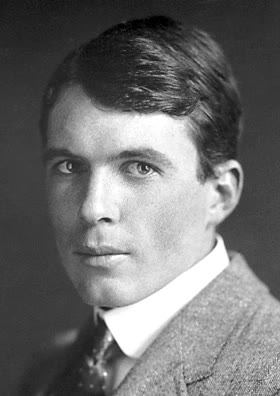
\includegraphics[width=\linewidth]{images/book4/bragg-wl.jpg}\par
{\footnotesize W. L. Bragg.}
\end{minipage}
\end{history}

\section{Exercices}

\begin{exercise}[$\star$]\label{exo:b3:x-ray-diffraction:1}
% ledger: lat:NaCl
Pour \ce{NaCl} ($a = \qty{564.06}{pm}$), calculer $d_{111}$, $d_{200}$ et $d_{220}$.
\end{exercise}

\begin{exercise}[$\star$]\label{exo:b3:x-ray-diffraction:2}
% ledger: lat:Cu, xray:CuKa1
Le cuivre est cubique à faces centrées avec $a = \qty{361.50}{pm}$. Avec
la raie Cu K$\alpha_1$ ($\lambda = \qty{154.06}{pm}$),
calculer $2\theta$ pour ses deux premières réflexions, après les avoir
nommées.
\end{exercise}

\begin{exercise}[$\star$]\label{exo:b3:x-ray-diffraction:3}
Lesquelles des réflexions 100, 110, 111, 200, 210, 211, 220 sont
présentes pour un réseau cubique P, I et F~?
\end{exercise}

\begin{exercise}[$\star$]\label{exo:b3:x-ray-diffraction:4}
Donner la base réciproque d'un réseau rectangulaire à deux dimensions de
côtés $a$ et $b$, et dessiner les premiers nœuds réciproques.
\end{exercise}

\begin{exercise}[$\star\star$]\label{exo:b3:x-ray-diffraction:5}
% ledger: lat:W
Un métal donne des raies à $2\theta = 40.27$, 58.26, 73.20, 87.01 et
\ang{100.66} avec la raie Cu
K$\alpha_1$. Indexer le diagramme, trouver le type de réseau et $a$.
\end{exercise}

\begin{exercise}[$\star\star$]\label{exo:b3:x-ray-diffraction:6}
% ledger: lat:KCl
Un cristal de \ce{KCl} ($a = \qty{629.29}{pm}$) a une masse volumique
mesurée de
\qty{1.99}{g/cm^3} (données de l'exercice). Trouver $Z$.
\end{exercise}

\begin{exercise}[$\star\star$]\label{exo:b3:x-ray-diffraction:7}
La raie (200) d'une nanopoudre de \ce{NaCl} ($2\theta = \ang{31.70}$) a
une largeur de \ang{0.40}, la contribution instrumentale étant nulle.
Estimer la taille des cristallites.
\end{exercise}

\begin{exercise}[$\star\star$]\label{exo:b3:x-ray-diffraction:8}
\ce{CsCl} a \ce{Cs+} en $(0,0,0)$ et \ce{Cl-} en $(\frac12,\frac12,\frac12)$ dans une maille P. Avec $f
\approx$ le nombre d'électrons, calculer $F_{100}$ et $F_{110}$ et le
rapport de leurs intensités (\omterm{def:b3:x-ray-diffraction:structure-factor}{facteur de structure} seul). Pourquoi
\ce{CsCl} n'est-il pas cubique centré~?
\end{exercise}

\begin{exercise}[$\star\star$]\label{exo:b3:x-ray-diffraction:9}
Montrer qu'un réseau à bases centrées C (nœud supplémentaire en
$(\frac12,\frac12,0)$) éteint les
réflexions telles que $h + k$ est impair.
\end{exercise}

\begin{exercise}[$\star\star\star$]\label{exo:b3:x-ray-diffraction:10}
Expliquer pourquoi la découverte, dans les années 1980, d'alliages dont
les diagrammes de diffraction présentent des taches nettes de symétrie
d'ordre dix n'a pas contredit la restriction cristallographique, et ce
qu'elle a changé dans la définition d'un cristal.
\end{exercise}

\begin{exercise}[$\star\star\star$]\label{exo:b3:x-ray-diffraction:11}
Montrer que dans \textit{P}$2_1/c$ le \omterm{def:b3:x-ray-diffraction:space-group}{plan de glissement} éteint les
réflexions $h0l$ avec $l$
impair.
\end{exercise}

\begin{exercise}[$\star\star\star$]\label{exo:b3:x-ray-diffraction:12}
Un énantiomère pur ne peut jamais cristalliser dans un \omterm{def:b3:x-ray-diffraction:space-group}{groupe d'espace}
contenant un \omterm{def:b3:point-groups:inversion}{centre d'inversion}, un miroir ou un \omterm{def:b3:x-ray-diffraction:space-group}{plan de glissement}.
Pourquoi~? À quel type de \omterm{def:b3:x-ray-diffraction:space-group}{groupes d'espace} est-il restreint, et
qu'implique la loi de Friedel pour la détermination de sa configuration
absolue~?
\end{exercise}

% keep the heading with its problem box, which fills a page by itself
\clearpage
\enlargethispage{3\baselineskip}
\section{Problème~: quelle poudre blanche~?}

\begin{problem}[{Problème du week-end --- le diagramme de poudre d'un sel
cubique inconnu~: distances, indexation, paramètre de maille, identité
du sel, taille des cristallites}]
\label{pb:b3:x-ray-diffraction:1}
% ledger: xray:CuKa1, lat:NaCl, lat:KCl, lat:KBr
Une poudre cristalline blanche inconnue, dont on sait qu'il s'agit de
\ce{NaCl}, de \ce{KCl} ou de \ce{KBr},
donne avec le rayonnement Cu K$\alpha_1$ ($\lambda = \qty{154.059}{pm}$)
les raies suivantes (données du problème, calculées pour cet exercice)~:
\begin{center}\small
\begin{tabular}{lcccccc}
\hline
$2\theta$ / degré & 28.342 & 40.512 & 50.178 & 58.632 & 66.380 & 73.692 \\
intensité relative & 100 & 92 & 38 & 20 & 61 & 49 \\ \hline
\end{tabular}
\end{center}
Aucune autre raie n'apparaît entre 20 et \ang{75}. Paramètres de maille
de référence~:
\ce{NaCl} \qty{564.06}{pm}, \ce{KCl} \qty{629.29}{pm}, \ce{KBr} \qty{658.47}{pm}. Masses
molaires~:
K 39.1, Na 23.0, Cl 35.5, Br \qty{79.9}{g/mol}.

\medskip\noindent\textbf{Partie I --- Les distances.}
\begin{enumerate}
  \item Calculer $\theta$ et $d$ pour la première raie.
  \item Calculer $d$ pour toutes les raies.
  \item Calculer les rapports $\sin^2\theta/\sin^2\theta_1$.
  \item Quelle suite d'entiers trouve-t-on~?
  \item Le diagramme pourrait-il être celui d'un réseau cubique
        primitif~? Avec quel $a$~?
  \item Pour un réseau cubique primitif, quel entier $N$ ne peut jamais
        apparaître~? Le diagramme permet-il à ce stade de départager les
        deux interprétations~?
\end{enumerate}

\medskip\noindent\textbf{Partie II --- Le réseau réel.}
\begin{enumerate}[resume]
  \item Les trois candidats sont des réseaux F. Indexer les raies avec la
        suite F.
  \item En déduire $a$ à partir de la première raie.
  \item Quel candidat convient~?
  \item Pour ce sel, pourquoi les réflexions à indices tous impairs (111),
        (311) sont-elles absentes~?
  \item \ce{NaCl} présenterait-il (111)~? Et \ce{KBr}~?
  \item Expliquer pourquoi l'interprétation primitive de la partie I est
        un piège.
\end{enumerate}

\medskip\noindent\textbf{Partie III --- Masse volumique et contenu.}
\begin{enumerate}[resume]
  \item Combien de groupements formulaires la maille contient-elle~?
  \item Calculer la masse volumique à partir de la maille.
  \item Donner la coordinence de chaque ion.
  \item Calculer la plus courte distance K--Cl.
  \item Quelle réflexion apparaîtrait la première au-delà de \ang{75}~?
  \item Pourquoi les intensités sont-elles moins utiles que les positions
        pour identifier une phase~?
\end{enumerate}

\medskip\noindent\textbf{Partie IV --- Affinement et taille des cristallites.}
\begin{enumerate}[resume]
  \item Pourquoi tirer le paramètre de maille d'une raie aux grands
        angles~?
  \item Calculer $a$ à partir de la raie (420).
  \item La raie (420) a une largeur de \ang{0.25} en $2\theta$ (largeur
        instrumentale négligeable). Estimer la taille des cristallites.
  \item Une taille de cristallites de \qty{1}{\micro m} élargirait-elle la
        raie de façon mesurable~?
  \item Énoncer le résultat~: paramètre de maille affiné sur la raie
        (420) et identité de la poudre.
\end{enumerate}
\end{problem}
